\chapter{Description Logics}
\label{cha:description-logics}

In this section, we shall introduce some basic notions of description logics as they are
needed for the purpose of this work.  This shall include a discussion of some of the basic
\emph{syntax} and \emph{semantics} of description logics
(Section~\ref{sec:basic-noti-descr}), as well as a discussion of \emph{knowledge bases}
and \emph{standard reasoning tasks} (Section~\ref{sec:knowledge-bases}).

Our focus in this work will be upon the light-weight description logic \ELbot, which shall
be the target logic for the knowledge we want to extract from data.  However, at a later
point in this work we shall see that the expressivity of \ELbot is not sufficient for our
needs, and that we need to consider an extension of \ELbot instead.  This extension shall
be the logic \ELgfpbot, an extension of \ELbot by \emph{greatest fixpoint semantics}.  We
shall therefore also include an introduction to the syntax and semantics of \ELgfpbot in
this chapter.  This will be done in Section~\ref{sec:descr-logics-elbot}.

\section{Syntax and Semantics of the Description Logic \ELbot}
\label{sec:basic-noti-descr}

We start our introduction to description logics by defining the syntax of the description
logic \ELbot, one of the simplest and least-expressive description logics under
consideration.  To this end, we choose two disjoint sets $N_C$ and $N_R$, called the sets
of \emph{concept names} and \emph{role names}, respectively.  Based upon this choice, we
introduce \emph{\ELbot concept descriptions} over $N_C$ and $N_R$ as follows.
\begin{Definition}[\ELbot Concept Description]
  \label{def:ELbot-concept-descriptions}
  Let $N_C$ and $N_R$ be two disjoint sets.  An \emph{\EL concept description} $C$ (over
  $N_C$ and $N_R$) is of the form
  \begin{itemize}
  \item $C = A$ for some $A \in N_C$, or
  \item $C = C_1 \sqcap C_2$ for $C_1, C_2$ two \EL concept descriptions, or
  \item $C = \exists r. D$ for an \EL concept description $D$ and $r \in N_R$, or
  \item $C = \top$.
  \end{itemize}
  The constructors are called \emph{conjunction} ($\sqcap$), \emph{existential
    restriction} ($\exists$) and the \emph{top concept} ($\top$), respectively.

  An \ELbot concept description $C$ (over $N_C$ and $N_R$) is then either an \EL concept
  description or $C$ is of the form $C = \bot$.
\end{Definition}

We shall occasionally denote the set of all \EL concept descriptions over $N_C$ and $N_R$
by $\EL(N_C, N_R)$, and the set of all \ELbot concept descriptions over $N_C$ and $N_R$ by
$\ELbot(N_C, N_R)$.  The same is true for other description logics which we shall
introduce at a later point.  We shall also often talk just about \enquote{concept
  descriptions} without explicitly mentioning the description logic we are using.  If this
is the case, then any description logic introduced in this work can be used there.

The sets $N_C$ and $N_R$ of concept and role names are also called the \emph{signature} of
the logic.  In the following we shall always assume that those sets are finite.  Sometimes
this signature is extended by another set $N_I$ called the set of \emph{individual names}.
Such individual names allow a logic to directly refer to individual elements of a domain.
However, this expressiveness is not available in the description logics \EL and \ELbot,
but we shall nevertheless include them in our further discussion as they are needed to
define the semantics of assertional axioms.  See also Section~\ref{sec:knowledge-bases}.

\begin{Example}
  \label{expl:tom-and-jerry-1}
  Let $N_C := \set{ \mathsf{Cat}, \mathsf{Mouse} }$ and let $N_R := \set{ \mathsf{hunts}
  }$.  Then examples of \ELbot concept descriptions would be
  \begin{equation*}
    \mathsf{Cat}, \, \mathsf{\exists hunts. Mouse}, \, \mathsf{Cat \sqcap Mouse}, \, \bot.
  \end{equation*}
  One can think of these concept descriptions as \enquote{describing} things in a certain
  domain (we shall make this much more precise shortly).  For example, the concept
  description $\mathsf{Cat}$ describes everything which is a cat.  The concept description
  $\mathsf{\exists hunts. Mouse}$ describes everything which hunts a mouse (alternatively:
  a thing that hunts something which is a mouse).  The concept description $\mathsf{Cat
    \sqcap Mouse}$ describes things that are both a cat and a mouse.  Finally, the concept
  description $\bot$ just describes nothing.
\end{Example}

The intuition of a concept description to \enquote{describe things} conveyed in the
previous example is very vague, and we shall make it more precise by introducing the
notion of an \emph{interpretation}.

\begin{Definition}[Interpretation]
  \label{def:interpretation}
  Let $N_C$ and $N_R$ be two disjoint sets.  Let $N_I$ be another set, disjoint to both
  $N_{C}$ and $N_{R}$, called the set of \emph{individual names}.  An
  \emph{interpretation} $\mathcal{I} = (\Delta^{\mathcal{I}}, \cdot^{\mathcal{I}})$ (over
  $N_C$, $N_R$ and $N_I$) consists of a nonempty set $\Delta^{\mathcal{I}}$ of
  \emph{elements}, and an \emph{interpretation function} $\cdot^{\mathcal{I}}$ such that
  \begin{enumerate}[i. ]
  \item $A^{\mathcal{I}} \subseteq \Delta^{\mathcal{I}}$ for all $A \in N_C$,
  \item $r^{\mathcal{I}} \subseteq \Delta^{\mathcal{I}} \times \Delta^{\mathcal{I}}$ for
    all $r \in N_R$, and
  \item $a^{\mathcal{I}} \in \Delta^{\mathcal{I}}$ for all $a \in N_I$.
  \end{enumerate}
  We furthermore make the \emph{unique name assumption}: if $a, b \in N_I$ and $a \neq b$,
  then $a^{\mathcal{I}} \neq b^{\mathcal{I}}$.

  We say that $\mathcal{I}$ is finite if $\Delta^{\mathcal{I}}$ is finite.
\end{Definition}

If the set $N_I$ in the definition of an interpretation is not important for the current
consideration, then we shall set $N_I = \emptyset$ and just speak of an interpretation
over $N_C$ and $N_R$.

\begin{Example}
  \label{expl:tom-hunts-jerry-hunts-tom-interpretation}
  Let us consider an example interpretation $\mathcal{I}_{\mathsf{MGM}}$ for our signature
  $N_C = \set{ \mathsf{Cat}, \mathsf{Mouse} }$ and $N_R = \set{ \mathsf{hunts} }$.  For
  this we set
  \begin{equation*}
    \mathcal{I}_{\mathsf{MGM}} := (\set{ \mathsf{tom}, \mathsf{jerry} }, \cdot^{\mathcal{I}_{\mathsf{MGM}}})
  \end{equation*}
  where
  \begin{align*}
    \mathsf{Cat}^{\mathcal{I}_{\mathsf{MGM}}} &= \set{ \mathsf{tom} }, \\
    \mathsf{Mouse}^{\mathcal{I}_{\mathsf{MGM}}} &= \set{ \mathsf{jerry} }, \\
    \mathsf{hunts}^{\mathcal{I}_{\mathsf{MGM}}} &= \set{ (\mathsf{tom}, \mathsf{jerry}),
      (\mathsf{jerry}, \mathsf{tom}) }.
  \end{align*}
  The interpretation $\mathcal{I}_{\mathsf{MGM}}$ can naturally be represented as a graph,
  where we consider the elements of $\Delta^{\mathcal{I}_{\mathsf{MGM}}}$ as vertices and
  the pairs in $\mathsf{hunts}^{\mathcal{I}_{\mathsf{MGM}}}$ as directed edges:
  \begin{center}
    \begin{tikzpicture}
      \begin{scope}[every node/.style = { draw, circle }]
        \node (Tom) {\textsf{tom}};
        \node[right=2cm of Tom, inner sep = .1cm] (Jerry) {\textsf{jerry}}; % fix
      \end{scope}
      \path (Tom) edge[->, bend left=30] node[midway, above] {\textsf{hunts}} (Jerry);
      \path (Jerry) edge[->, bend left=30] node[midway, below] {\textsf{hunts}} (Tom);
    \end{tikzpicture}
  \end{center}
\end{Example}

The interpretation function of a given interpretation can now be naturally extended to the
set of \EL and \ELbot concept descriptions.

\begin{Definition}[Extensions]
  \label{def:extending-the-interpretation-function}
  Let $\mathcal{I} = (\Delta^{\mathcal{I}}, \cdot^{\mathcal{I}})$ be an interpretation.
  Then the \emph{extension} of $\cdot^{\mathcal{I}}$ to all \ELbot concept descriptions is
  inductively defined as follows: let $C_1, C_2, C \in \ELbot(N_C, N_R)$ and $r \in N_R$.
  Then
  \begin{enumerate}[i. ]
  \item $\top^{\mathcal{I}} = \Delta^{\mathcal{I}}$,
  \item $\bot^{\mathcal{I}} = \emptyset$,
  \item $(C_1 \sqcap C_2)^{\mathcal{I}} := C_1^{\mathcal{I}} \cap C_2^{\mathcal{I}}$, and
  \item $(\exists r. C)^{\mathcal{I}} := \set{ x \in \Delta^{\mathcal{I}} \mid \exists y
      \in \Delta^{\mathcal{I}} \st (x, y) \in r^{\mathcal{I}} \land y \in C^{\mathcal{I}} }$.
  \end{enumerate}
  We shall call the set $C^{\mathcal{I}}$ the \emph{extension} of $C$ in $\mathcal{I}$.
\end{Definition}

The notion of an extension of an \ELbot concept description in an interpretation now
formalizes our previous intuitive understanding that concept descriptions
\enquote{describe things:} an element $x \in \Delta^{\mathcal{I}}$ is described by an
\ELbot concept description $C$ in $\mathcal{I}$ if and only if $x \in C^{\mathcal{I}}$.

\begin{Example}
  \label{expl:tom-and-jerry-2}
  Let us consider the example interpretation $\mathcal{I}_{\mathsf{MGM}}$ from
  Example~\ref{expl:tom-hunts-jerry-hunts-tom-interpretation} again, and let us compute
  for the example \ELbot concept descriptions from Example~\ref{expl:tom-and-jerry-1}
  their extensions.  We obtain
  \begin{align*}
    (\mathsf{\exists hunts. Mouse})^{\mathcal{I}_{\mathsf{MGM}}} &= \set{ x \in
      \Delta^{\mathcal{I}_{\mathsf{MGM}}} \mid \exists y \in
      \Delta^{\mathcal{I}_{\mathsf{MGM}}} \st (x, y) \in
      \mathsf{hunts}^{\mathcal{I}_{\mathsf{MGM}}} \land y \in
      \mathsf{Mouse}^{\mathcal{I}_{\mathsf{MGM}}} }\\
    &= \set{ \mathsf{tom} } = \mathsf{Cat}^{\mathcal{I}_{\mathsf{MGM}}},\\
    \mathsf{Cat \sqcap Mouse}^{\mathcal{I}_{\mathsf{MGM}}}
    &= \emptyset = \bot^{\mathcal{I}_{\mathsf{MGM}}}.
  \end{align*}
\end{Example}

For some \ELbot concept descriptions $C, D$ it may be the case that \emph{for all}
interpretations $\mathcal{I}$ it is true that
\begin{equation*}
  C^{\mathcal{I}} \subseteq D^{\mathcal{I}}.
\end{equation*}
In this case, we say that $C$ is \emph{subsumed by} $D$, and write $C \sqsubseteq D$.  If
$C$ is subsumed by $D$ and, in addition, $D$ is subsumed by $C$, then for all
interpretations $\mathcal{I}$ it is true that $C^{\mathcal{I}} = D^{\mathcal{I}}$.  In
this case we say that $C$ and $D$ are \emph{equivalent}.  In this case, we shall write $C
\equiv D$.

The definitions we have given so far only apply to the description logics \EL and \ELbot,
which are of course not the only ones.  Another notable description logic is $\ALC$, a
description logic that provides for conjunction, disjunction, negation, $\top$, $\bot$ as
well as existential and value restrictions.  The definition of the syntax of \ALC is
analogous to the one for \EL.  The semantics of \ALC is again based on interpretations,
and the corresponding extension of the interpretation function to all \ALC concept
descriptions is given in Table~\ref{tab:ALC-syntax}.

\begin{table}[tp]
  \centering
  \renewcommand{\arraystretch}{1.2}
  \begin{tabular}[c]{l l l}
    \toprule
    Constructor Name         & Syntax           & Semantics \\
    \midrule
    top concept              & $\top$           & $\Delta^{\mathcal{I}}$ \\
    bottom concept           & $\bot$           & $\emptyset$ \\
    conjunction              & $C_1 \sqcap C_2$ & $C_1^{\mathcal{I}} \cap C_2^{\mathcal{I}}$ \\
    disjunction              & $C_1 \sqcup C_2$ & $C_1^{\mathcal{I}} \cup C_2^{\mathcal{I}}$ \\
    existential restriction  & $\exists r. C$   & $\set{ x \in \Delta^{\mathcal{I}} \mid
      \exists y \in \Delta^{\mathcal{I}} \st (x, y) \in r^{\mathcal{I}} \land y \in
      C^{\mathcal{I}} }$ \\
    value restriction        & $\forall r. C$   & $\set{ x \in \Delta^{\mathcal{I}} \mid
      \forall y \in \Delta^{\mathcal{I}} \holds (x, y) \in r^{\mathcal{I}} \implies y \in
      C^{\mathcal{I}} }$ \\
    negation                 & $\neg C$         & $\Delta^{\mathcal{I}} \setminus
    C^{\mathcal{I}}$ \\
    \bottomrule
  \end{tabular}
  \caption{Syntax Constructors of \ALC}
  \label{tab:ALC-syntax}
\end{table}

\ALC usually serves as a touchstone for the expressivity of a description logic: a
description logic is usually called \emph{inexpressive} if it does not provide (directly
or indirectly) all constructors of \ALC.  A description logic which provides all
constructors of \ALC is usually called \emph{expressive}.

Additionally, \ALC played a crucial role in the development of description logics by
uncovering a close connection to \emph{modal
  logics}~\cite{MLhandbook,BaaderLutz-MLhandbook-06}: in~\cite{DBLP:conf/ijcai/Schild91}
it was shown that \ALC can be considered as a syntactic variant of the multimodal logic
$\mathsf{K}_{(\mathsf{m})}$.

\section{Knowledge Bases and Reasoning}
\label{sec:knowledge-bases}

Having defined a description logic, one can use it to state \emph{axioms}.  These axioms
can be of different nature: they can either state facts about individuals, or they can
state facts about concept descriptions in general.  In the former case, axioms are called
\emph{assertional axioms}, in the latter case they are called \emph{terminological
  axioms}.  A \emph{knowledge base} (or \emph{ontology}) $\mathcal{K} = (\mathcal{T},
\mathcal{A})$ then consists of those axioms, where the assertional axioms are collected
into an \emph{ABox} $\mathcal{A}$, and where the terminological axioms are collected into
a \emph{TBox} $\mathcal{T}$.

If then one has given such a knowledge base $\mathcal{K}$, one can conduct \emph{reasoning}
with it.  Essentially, reasoning is the extraction of knowledge which is \emph{entailed}
by the knowledge base $\mathcal{K}$.  Of course, for this to make sense we need to define
a semantics for the knowledge base $\mathcal{K}$.  Standard reasoning tasks are then
\emph{subsumption}, \emph{instance checking}, \emph{consistency checking} and
\emph{satisfiability}.

Let us start by formally introducing the notions of \emph{assertional axioms} and
\emph{ABoxes}.

\begin{Definition}[Assertional Axiom, ABox]
  \label{def:assertional-axiom-and-ABox}
  Let $N_C$, $N_R$ and $N_I$ be three pairwise disjoint sets.  An \emph{assertional axiom}
  (over $N_C$, $N_R$ and $N_I$) is an expression of the form
  \begin{equation*}
    C(a) \quad\text{or}\quad r(a, b)
  \end{equation*}
  where $a, b \in N_I, r \in N_R$ and $C \in \ELbot(N_C, N_R)$ is an \ELbot concept
  description.  An assertional axiom $C(a)$ and $r(a,b)$ \emph{holds} in an interpretation
  $\mathcal{I}$, written as $\mathcal{I} \models C(a)$ and $\mathcal{I} \models r(a, b)$,
  if and only if
  \begin{align*}
    a^{\mathcal{I}} \in C^{\mathcal{I}} \quad\text{and}\quad (a^{\mathcal{I}},
    b^{\mathcal{I}}) \in r^{\mathcal{I}},
  \end{align*}
  respectively.  An \emph{ABox} $\mathcal{A}$ is then just a set of assertional axioms
  (over $N_C$, $N_R$ and $N_I$).  An interpretation $\mathcal{I}$ is a \emph{model} of an
  ABox $\mathcal{A}$, written $\mathcal{I} \models \mathcal{A}$ if and only if every
  assertional axiom in $\mathcal{A}$ holds in $\mathcal{I}$.
\end{Definition}

\begin{Example}
  \label{expl:tom-and-jerry-ABox}
  Let us consider Example~\ref{expl:tom-and-jerry-1} again, and let us consider some
  assertional axioms over $N_C$, $N_R$ and $N_I$.  For example we can state that
  \textsf{tom} is a \textsf{Cat}, \textsf{jerry} is a \textsf{Mouse}, that \textsf{tom}
  \textsf{hunts} \textsf{jerry} and that \textsf{jerry} \textsf{hunts} \textsf{tom}.  This
  can be achieved (in that order) with the following ABox:
  \begin{equation*}
    \mathcal{A}_{\mathsf{MGM}} = \set{ \mathsf{Cat}(\mathsf{tom}), \mathsf{Mouse}(\mathsf{jerry}),
      \mathsf{hunts}(\mathsf{tom}, \mathsf{jerry}),
      \mathsf{hunts}(\mathsf{jerry}, \mathsf{tom}) }.
  \end{equation*}
  The interpretation $\mathcal{I}_{\mathsf{MGM}}$ from
  Example~\ref{expl:tom-hunts-jerry-hunts-tom-interpretation} is a model of
  $\mathcal{A}_{\mathsf{MGM}}$, \ie $\mathcal{I}_{\mathsf{MGM}} \models
  \mathcal{A}_{\mathsf{MGM}}$.
\end{Example}

Complementary to assertional axioms are \emph{terminological axioms}, which state
connections between concept descriptions.  As already stated, they are collected into
\emph{TBoxes}.  However, in contrast to ABoxes, there are a lot of different kinds of
TBoxes.  We shall restrict our attention to two of these, namely \emph{cyclic} TBoxes and
\emph{general} TBoxes.  For the latter, we shall also introduce the notion of
\emph{general concept inclusions}, which is crucial for our further considerations.

\begin{Definition}[Concept Definitions, Cyclic TBoxes]
  \label{def:concept-definitions-cyclic-TBoxes}
  Let $N_C$ and $N_R$ be two disjoint sets, and let $N_D$ be another set disjoint to both
  $N_C$ and $N_R$.  A \emph{concept definition} (over $N_C, N_R$ and $N_D$) is an
  expression of the form
  \begin{equation*}
    B \equiv D
  \end{equation*}
  where $B \in N_D$ and $D$ is a concept description over $N_C \cup N_D$ and $N_R$.  The
  element $B$ is called the \emph{left-hand side} and the concept description $D$ is
  called the \emph{right-hand side} of the concept definition, respectively.

  A \emph{cyclic TBox} $\mathcal{T}$ (over $N_C, N_R$ and $N_D$) is a set consisting of
  concept definitions over $N_C$, $N_R$ and $N_D$ which additionally satisfies the
  condition that for every $B \in N_D$ there exists exactly one concept definition in
  $\mathcal{T}$ with $B$ on the left-hand side.  The set $N_D$ is called the set of
  \emph{defined concept names} of $\mathcal{T}$, and is also denoted by
  $N_D(\mathcal{T})$.

  A concept definition $B \equiv D$ is said to \emph{hold} in an interpretation
  $\mathcal{I}$ over $N_C \cup N_D$ and $N_R$, written $\mathcal{I} \models (B \equiv D)$,
  if and only if
  \begin{equation*}
    B^{\mathcal{I}} = D^{\mathcal{I}}
  \end{equation*}
  is true.  The interpretation $\mathcal{I}$ is a \emph{model} for a cyclic TBox
  $\mathcal{T}$, written $\mathcal{I} \models \mathcal{T}$, if and only if every concept
  definition in $\mathcal{T}$ holds in $\mathcal{I}$.
\end{Definition}

A concept definition $B \equiv D$ is true in some interpretation $\mathcal{I}$ if and only
if $B^{\mathcal{I}} = D^{\mathcal{I}}$.  However, in some cases it may not be possible to
exactly define a concept name $B$ in terms of another concept description $D$.  In such
cases one can make use of \emph{general concept inclusions}: instead of requiring
$B^{\mathcal{I}} = D^{\mathcal{I}}$ one can equivalently state that
\begin{equation*}
  B^{\mathcal{I}} \subseteq D^{\mathcal{I}} \quad\text{and}\quad B^{\mathcal{I}} \supseteq D^{\mathcal{I}}.
\end{equation*}
If $B$ cannot be defined exactly, at least one of these inclusions may be true.  The way
to express this is to use general concept inclusion.

\begin{Definition}[General Concept Inclusion, General TBox]
  \label{def:general-concept-inclusions-and-general-TBoxes}
  Let $N_C$ and $N_R$ be two disjoint sets.  A \emph{general concept inclusion} (GCI) $C
  \sqsubseteq D$ (over $N_C$ and $N_R$) consists of two concept descriptions $C, D$ over
  $N_C$ and $N_R$.  A GCI $C \sqsubseteq D$ is said to \emph{hold} in an interpretation
  $\mathcal{I}$ if and only if $C^{\mathcal{I}} \subseteq
  D^{\mathcal{I}}$.\footnote{Notice that there is a possibility for confusion here: recall
    that we write $C \sqsubseteq D$ if $C$ is subsumed by $D$.  So the fact that $C
    \sqsubseteq D$ could potentially be confused with the general concept inclusion $C
    \sqsubseteq D$.  However, the former is a statement, while the latter is an
    expression, so confusing those two is rather unlikely.}

  A collection $\mathcal{T}$ of general concept inclusions is called a \emph{general
    TBox}.  An interpretation $\mathcal{I}$ is said to be a \emph{model} of the general
  TBox $\mathcal{T}$, written $\mathcal{I} \models \mathcal{T}$, if and only if every GCI
  $(C \sqsubseteq D) \in \mathcal{T}$ holds in $\mathcal{I}$.  In this case we shall also
  say that $C \sqsubseteq D$ is \emph{valid} in $\mathcal{I}$, or \emph{holds} in
  $\mathcal{I}$.
\end{Definition}

In the sense discussed above, concept definitions can be expressed in terms of general
concept inclusions.  Because of this representation, we can regard cyclic TBoxes as
special cases of general TBoxes.  Therefore, if we talk about TBoxes in the following we
mean either of these notions.

Knowledge bases are now just pairs consisting of an ABox and a TBox.
\begin{Definition}[Knowledge Base]
  \label{def:knowledge-base}
  Let $N_C, N_R$ and $N_I$ be pairwise disjoint sets.  Let $\mathcal{A}$ be an ABox over
  $N_C$, $N_R$ and $N_I$, and let $\mathcal{T}$ be a TBox over $N_C$ and $N_R$.  Then the
  pair
  \begin{equation*}
    \mathcal{K} = (\mathcal{T}, \mathcal{A})
  \end{equation*}
  is called a \emph{knowledge base} (or \emph{ontology}) (over $N_C$ and $N_R$).  An
  interpretation is a \emph{model} of $\mathcal{K}$ if and only if it is a model of both
  $\mathcal{T}$ and $\mathcal{A}$.
\end{Definition}

Knowledge bases are the core method of description logics to represent knowledge.  In the
following, we shall consider some of the standard reasoning tasks which can be conducted
as soon as a knowledge base is available.  As already mentioned, \emph{reasoning} can be
seen as the process to extract knowledge from a knowledge base which may be represented
only implicitly.  The following definitions shall make clear what we mean when we talk
about implicitly represented knowledge.

\begin{Definition}[Consistency Checking]
  \label{def:concistency-checking}
  Let $\mathcal{K}$ be a knowledge base.  The \emph{consistency checking problem} for
  $\mathcal{K}$ is to decide whether $\mathcal{K}$ has a model.
\end{Definition}

\begin{Definition}[Satisfiability Checking]
  \label{def:satisfiability-checking}
  Let $\mathcal{K}$ be a knowledge base, and let $C$ be an concept description.  The
  \emph{satisfiability checking problem} for $\mathcal{K}$ and $C$ is to decide whether
  $C$ is satisfiable with respect to $\mathcal{K}$, \ie whether there exists a model
  $\mathcal{I}$ of $\mathcal{K}$ such that $C^{\mathcal{I}} \neq \emptyset$.
\end{Definition}

Both checking for consistency and checking satisfiability of certain concept descriptions
may be helpful to detect errors in the knowledge base.

\begin{Definition}[Subsumption Checking]
  \label{def:subsumption-checking}
  Let $\mathcal{K}$ be a knowledge base, and let $C, D$ be two concept descriptions.  Then
  the \emph{subsumption checking problem} for $\mathcal{K}, C, D$ is to decide whether $C$
  is subsumed by $D$ with respect to $\mathcal{K}$, written $C \sqsubseteq_{\mathcal{K}}
  D$, which means to decide whether $C^{\mathcal{I}} \subseteq D^{\mathcal{I}}$ is true
  for all models $\mathcal{I}$ of $\mathcal{K}$.
\end{Definition}

Checking subsumption between concept descriptions helps to extract dependencies between
concept descriptions in all models of the knowledge base, even if those are not
represented explicitly.  A related reasoning task is \emph{classification}.

\begin{Definition}[Classification]
  \label{def:classification}
  Let $\mathcal{K}$ be a knowledge base over $N_{C}$ and $N_{R}$.  Then to \emph{classify}
  $\mathcal{K}$ means to compute the set of all general concept inclusions $A \sqsubseteq
  B$ such that $A \sqsubseteq_{\mathcal{K}} B$, where $A, B \in N_{C}$.
\end{Definition}

Classification and subsumption checking only treat the TBox of the knowledge base.  A
reasoning task which also involves the ABox is \emph{instance checking}, which may be
utilized to find errors in the knowledge base that are related to individuals.

\begin{Definition}[Instance Checking]
  \label{def:instance-checking}
  Let $\mathcal{K}$ be a knowledge base, let $C$ be a concept description, and let $a$ be
  an individual name.  Then the \emph{instance checking problem} for $\mathcal{K}, C, a$
  is to decide if $a$ is an instance of $C$ with respect to $\mathcal{K}$, \ie whether in
  all models $\mathcal{I}$ of $\mathcal{K}$ it is true that $a^{\mathcal{I}} \in
  C^{\mathcal{I}}$.
\end{Definition}

The complexity of deciding the above decision problems of consistency, satisfiability,
subsumption and instance checking is usually used to measure the \emph{reasoning
  complexity} of a description logic.  For expressive description logics it is easy to see
that all problems can be reduced to \emph{instance checking}.  To this end, let
$\mathcal{K} = (\mathcal{T}, \mathcal{A})$ be a knowledge base.  Then
\begin{enumerate}[i. ]
\item $\mathcal{K}$ is consistent if and only if $a$ is not an instance of $\bot$ for an
  arbitrarily chosen individual name $a$;
\item $C$ is satisfiable with respect to $\mathcal{K}$ if and only if $(\mathcal{T},
  \mathcal{A} \cup \set{ C(a) } )$ is consistent, for some individual name $a$ which does
  not appear in $\mathcal{A}$;
\item $C$ is subsumed by $D$ with respect to $\mathcal{K}$ if and only if $C \sqcap \neg
  D$ is not satisfiable with respect to $\mathcal{K}$.
\end{enumerate}
For logics like \ALC it is therefore sufficient to know the complexity of the instance
checking problem to know the complexity of the other problems.  The instance problem is
ExpTime-complete for \ALC~\cite{DLhandbook}, and if the TBox of the knowledge base is
empty, the complexity of instance checking is PSpace-complete.

For \ELbot the above reductions do not work anymore, as negation is not available there,
and the complexity of the above reasoning problems has more or less to be established
separately.  It has been shown in~\cite{DBLP:conf/ijcai/Baader03a,
  DBLP:conf/ecai/Brandt04, DBLP:conf/ijcai/BaaderBL05} that all the above mentioned
reasoning problems are tractable, \ie in PTime.

It is worth noting that \ALC, as a variant of the multimodal logic
$\mathsf{K}_{(\mathsf{m})}$, has the so-called \emph{finite model property}: if
$\mathcal{K}, C$ is an instance of the satisfiability checking problem, then $C$ is
satisfiable with respect to $\mathcal{K}$ if and only if there exists a \emph{finite}
model $\mathcal{I}$ of $\mathcal{K}$ such that $C^{\mathcal{I}} \neq \emptyset$.  This
also implies that the subsumption problem can be decided over finite models only: if
$C^{\mathcal{I}} \subseteq D^{\mathcal{I}}$ holds for all finite models $\mathcal{I}$ of
$\mathcal{K}$, then $C \sqcap \neg D$ is not satisfiable over some finite model of
$\mathcal{K}$.  Because of the finite model property of \ALC, this implies that $C \sqcap
\neg D$ is not satisfiable over any model of $\mathcal{K}$, and thus $C$ is subsumed by
$D$ with respect to $\mathcal{K}$.  Observe that since \ELbot is a sub-logic of \ALC, it
also has the finite model property.

Apart from the standard reasoning tasks, there are many other reasoning problems connected
to knowledge bases, like \emph{axiom pinpointing}~\cite{DBLP:phd/de/Nyssen2009a} and
\emph{modularization}~\cite{conf/www/GrauHKS07}.  A task that is interesting also for our
considerations is the computation of \emph{least common
  subsumers}~\cite{phd/de/Turhan2007,conf/ijcai/BaaderKM99}.

\begin{Definition}[Least Common Subsumer]
  \label{def:least-common-subsumer}
  Let $C_1, \dots, C_n$ be concept descriptions, and let $D$ be another concept
  description such that
  \begin{enumerate}[i. ]
  \item $C_i \sqsubseteq D$ for $i = 1, \dots, n$ and
  \item for every concept description $E$ such that $C_i \sqsubseteq E$ is true for all $i
    = 1, \dots, n$, it is also true that $D \sqsubseteq E$.
  \end{enumerate}
  Then $D$ is called the \emph{least common subsumer} of $C_{1}, \dots, C_{n}$.
\end{Definition}

If least common subsumers exist they are unique up to equivalence: if $D_1$ and $D_2$ are
least common subsumers of $C_1, \dots, C_n$, then by the second condition of the
Definition~\ref{def:least-common-subsumer} it is true that $D_1 \sqsubseteq D_2$ and $D_2
\sqsubseteq D_1$, \ie $D_1 \equiv D_2$.  We shall denote the least common subsumer of
$C_1, \dots, C_n$ by $\lcs(\set{C_1, \dots, C_n})$.

Least common subsumers always exist in \EL and \ELbot, \ie if all concept descriptions
mentioned in Definition~\ref{def:least-common-subsumer} are either \EL concept
descriptions or \ELbot concept descriptions, then the least common subsumer always
exists~\cite{conf/ijcai/BaaderKM99}.

\section{The Description Logic \ELgfpbot}
\label{sec:descr-logics-elbot}

For our considerations on extracting general concept inclusions from finite
interpretations we shall soon see that the expressivity of \ELbot is not sufficient
anymore.  In particular, we shall see that in \ELbot \emph{model-based most-specific
  concept descriptions} do not necessarily exist.  These are concept descriptions $C$
which are \emph{most specific} in describing a certain set of individuals $X$ in an
interpretation $\mathcal{I}$, \ie it is true that
\begin{enumerate}[i. ]
\item $X \subseteq C^{\mathcal{I}}$ and
\item for all concept descriptions $D$ such that $X \subseteq D^{\mathcal{I}}$ it is true
  that $C \sqsubseteq D$.
\end{enumerate}
We shall discuss model-based most-specific concept descriptions in much more detail in
Section~\ref{sec:motivation}.  Here we just show by means of an example that they do not
necessarily need to exist in \ELbot.

\begin{Example}
  \label{expl:mmscs-may-not-exist-in-ELbot}
  Let us consider $N_C = \emptyset, N_R = \set{ \mathsf{r} }$ and the interpretation
  $\mathcal{I} = (\set{\mathsf{a}}, \cdot^{\mathcal{I}})$ over $N_C$ and $N_R$, which is
  given by $r^{\mathcal{I}} = \set{ (\mathsf{a}, \mathsf{a}) }$.  When depicted as a
  graph, this interpretation is just a single node graph with a loop:
  \begin{center}
    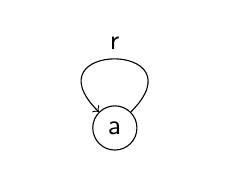
\begin{tikzpicture}
      \node[circle, draw] (a) {$\mathsf{a}$};
      \path[->] (a) edge[looseness=8] node[midway, above] {\textsf{r}} (a);
    \end{tikzpicture}
  \end{center}
  Let $X = \set{ \mathsf{a} }$.  Then we can find that \emph{all} \EL concept descriptions
  which can be formed over the vocabulary $N_C$ and $N_R$ describe $X$.  More
  specifically, all \EL concept descriptions which can be formed over $N_C$ and $N_R$ are
  of the form
  \begin{equation*}
    \exists \mathsf{r}^n. \top := \underbrace{\exists \mathsf{r}. \exists \mathsf{r}. \dots \exists
      \mathsf{r}}_{n \text{ times }}. \top
  \end{equation*}
  for $n \in \NN_0$.  But then for $m < n$ it is true that
  \begin{align*}
    \exists \mathsf{r}^{n}. \top &\sqsubseteq \exists \mathsf{r}^m. \top, \\
    \exists \mathsf{r}^{m}. \top &\not\sqsubseteq \exists \mathsf{r}^n. \top.
  \end{align*}
  Because of this, a most-specific concept description for $X$ does not exist.
\end{Example}

To remedy this deficit we shall consider an extension of \ELbot which does guarantee the
existence of model-based most-specific concept descriptions, namely the logic \ELgfpbot
which extends \ELbot by \emph{cyclic concept descriptions} and \emph{greatest fixpoint
  semantics}~\cite{DBLP:conf/ijcai/Baader03a,sowa/Nebel91}.

We shall start by introducing \emph{greatest fixpoint models} for cyclic TBoxes.  When we
introduced cyclic TBoxes $\mathcal{T}$ in \Cref{def:concept-definitions-cyclic-TBoxes}, we
have defined that an interpretation $\mathcal{I}$ is a model of $\mathcal{T}$ if and only
if every primitive concept description in $\mathcal{T}$ holds in $\mathcal{I}$.  This form
of semantics for cyclic TBoxes is called \emph{descriptive} semantics.  However, it is
possible to further restrict the notion of a model of $\mathcal{T}$, and such a
restriction is to use \emph{greatest fixpoint models} instead.  To introduce this
semantics we need some auxiliary definitions first.

\begin{Definition}[Primitive Interpretation, Extensions]
  \label{def:primite-interpretations-and-extentions}
  Let $\mathcal{T}$ be a cyclic TBox over $N_C$, $N_R$ and $N_D$.  We say that an
  interpretation $\mathcal{I} = (\Delta^{\mathcal{I}}, \cdot^{\mathcal{I}})$ is a
  \emph{primitive interpretation} for $\mathcal{T}$ if it is an interpretation over $N_C$
  and $N_R$, \ie $\cdot^{\mathcal{I}}$ assigns values to the concept names from $N_C$ but
  not to the defined concept names in $N_D$.  Another interpretation $\mathcal{J} =
  (\Delta^{\mathcal{J}}, \cdot^{\mathcal{J}})$ over $N_C \cup N_D$ and $N_R$ is said to
  \emph{extend} $\mathcal{I}$ if and only if $\mathcal{I}$ and $\mathcal{J}$ have the same
  set of elements and coincide on $N_C$ and $N_R$, \ie
  \begin{enumerate}[i. ]
  \item $\Delta^{\mathcal{I}} = \Delta^{\mathcal{J}}$,
  \item $A^{\mathcal{I}} = A^{\mathcal{J}}$ is true for all $A \in N_C$, and
  \item $r^{\mathcal{I}} = r^{\mathcal{J}}$ is true for all $r \in N_R$.
  \end{enumerate}
\end{Definition}

Based on this definition we can now give a characterization of models of cyclic TBoxes in
terms of fixpoints of certain functions.

Let $\mathcal{T}$ be a cyclic TBox over $N_C$, $N_R$ and $N_D$, and let $\mathcal{I}$ be a
primitive interpretation.  Let us denote with $\Ext(\mathcal{I})$ all interpretations over
$N_C \cup N_D$ and $N_R$ that extend $\mathcal{I}$.  Then we can naturally define an order
relation $\preceq$ on $\Ext(\mathcal{I})$ as follows: let $\mathcal{J}_1, \mathcal{J}_2
\in \Ext(\mathcal{I})$.  We define
\begin{equation*}
  \mathcal{J}_1 \preceq \mathcal{J}_2 \diff A^{\mathcal{J}_1} \subseteq A^{\mathcal{J}_2}
  \text{ for all } A \in N_D.
\end{equation*}
It can be seen quite easily that with this order relation the ordered set
$(\Ext(\mathcal{I}), \preceq)$ becomes a complete lattice: if $\set{ \mathcal{J}_i \mid i
  \in I } \subseteq \Ext(\mathcal{I})$, then $\sup \set{ \mathcal{J}_i \mid i \in I } =
\mathcal{J} \in \Ext(\mathcal{I})$, where
\begin{equation*}
  A^{\mathcal{J}} := \bigcup_{i \in I} A^{\mathcal{J}_i}
\end{equation*}
for all $A \in N_D$.  On this complete lattice we can now define an order-preserving map
$f_{\mathcal{I}} \colon \Ext(\mathcal{I}) \to \Ext(\mathcal{I})$ by means of the TBox
$\mathcal{T}$.  Let $\mathcal{J} \in \Ext(\mathcal{I})$.  We define
$f_{\mathcal{I}}(\mathcal{J}) = (\Delta^{\mathcal{I}},
\cdot^{f_{\mathcal{I}}(\mathcal{J})}) \in \Ext(\mathcal{I})$ by
\begin{equation*}
  A^{f_{\mathcal{I}}(\mathcal{J})} := C^{\mathcal{J}}
\end{equation*}
for all $(A \equiv C) \in \mathcal{T}$.  Note that since there exists for each $A \in N_D$
exactly one primitive concept definition $A \equiv C$ in $\mathcal{T}$, the function
$f_{\mathcal{I}}$ is well-defined.

Recall that $\mathcal{J} \in \Ext(\mathcal{I})$ is a model of $\mathcal{T}$ if and only if
\begin{equation*}
  A^{\mathcal{J}} = C^{\mathcal{J}}
\end{equation*}
holds for all $(A \equiv C) \in \mathcal{T}$.  We can rephrase this condition in terms of
\emph{fixpoints} of $f_{\mathcal{I}}$: since $A^{f_{\mathcal{I}}(\mathcal{J})} =
C^{\mathcal{J}}$, the interpretation $\mathcal{J}$ is a model of $\mathcal{T}$ if and only
if $\mathcal{J}$ is a fixpoint of $f_{\mathcal{I}}$, \ie $f(\mathcal{J}) = \mathcal{J}$.

As these fixpoints are elements of $\Ext(\mathcal{I})$, they are ordered by $\preceq$.
Therefore, intuitively, \emph{greatest fixpoint models} of $\mathcal{T}$ are just greatest
fixpoints of $f_{\mathcal{I}}$ with respect to $\preceq$.  To ensure their existence, we
need to invoke the fixpoint theorem by Tarski~\cite{Tarski-Fixpoint-Theorem}.

\begin{Theorem}
  \label{thm:tarski-fixpoint-theorem}
  Let $(L, \leq)$ be a complete lattice and let $f \colon L \to L$ be an order-preserving
  map, \ie
  \begin{equation*}
    x \leq y \implies f(x) \leq f(y)
  \end{equation*}
  is true for all $x, y \in L$.  Then the fixpoints form a complete sublattice of $(L,
  \leq)$, \ie the ordered set $(\set{ x \in L \mid f(x) = x }, \leq)$ is a complete
  lattice.  In particular, $\set{ x \in L \mid f(x) = x }$ is not empty and has greatest
  and smallest elements with respect to $\leq$.
\end{Theorem}

\begin{Definition}[Greatest Fixpoint Models]
  \label{def:gfp-models}
  Let $\mathcal{T}$ be a cyclic TBox over $N_C$, $N_R$ and $N_D$.  Let $\mathcal{I}$ be a
  primitive interpretation of $\mathcal{T}$.  An interpretation $\mathcal{J}$ over $N_C
  \cup N_D$ and $N_R$ is the \emph{greatest fixpoint model} of $\mathcal{T}$
  \emph{extending} $\mathcal{I}$ if and only if $\mathcal{J}$ is the greatest fixpoint of
  the mapping $f_{\mathcal{I}}$ defined as before.  An interpretation $\mathcal{J}$ over
  $N_C \cup N_D$ and $N_R$ is a \emph{greatest fixpoint model} of $\mathcal{T}$ if it is a
  greatest fixpoint model of $\mathcal{T}$ extending some primitive interpretation
  $\mathcal{I}$ of $\mathcal{T}$.
\end{Definition}

We continue our introduction of \ELgfpbot by discussing its semantics.  For this we
introduce the notion of a \emph{normalized} cyclic TBox.

\begin{Definition}[Normalized Cyclic TBox]
  \label{def:normalized-cyclic-TBox}
  Let $\mathcal{T}$ be a cyclic TBox over $N_C$, $N_R$ and $N_D$.  Then $\mathcal{T}$ is
  called \emph{normalized} if and only if for every primitive concept definition $(A
  \equiv C) \in \mathcal{T}$, the concept description $C$ is of the form
  \begin{equation*}
    C = P_1 \sqcap \dots \sqcap P_n \sqcap \exists r_1. A_1 \sqcap \dots \sqcap \exists r_m. A_m
  \end{equation*}
  for $n, m \in \NN_0$, $P_1, \dots, P_n \in N_C$, $r_1, \dots, r_m \in N_R$ and $A_1,
  \dots, A_m \in N_D$.
\end{Definition}

We finally have all notions available to define the syntax and semantics of \ELgfpbot.

\begin{Definition}[\ELgfpbot Concept Descriptions, \ELgfpbot Semantics]
  \label{def:ELgfpbot-concept-descriptions-and-their-semantics}
  Let $N_C$ and $N_R$ be two disjoint sets.  An \emph{\ELgfp concept description} is an
  expression of the form $C = (A, \mathcal{T})$, where $\mathcal{T}$ is a normalized
  cyclic TBox over $N_C$, $N_R$ and $N_D$, for some set $N_D$ disjoint to both $N_C$ and
  $N_R$, $\mathcal{T}$ only contains \EL concept descriptions, and $A \in N_D$.  An
  \emph{\ELgfpbot concept description} is either of the form $\bot$ or is an \ELgfp
  concept description.

  Let $\mathcal{I}$ be an interpretation over $N_{C}$ and $N_{R}$, and let $C = (A,
  \mathcal{T})$ be an \ELgfpbot concept description.  Then
  \begin{equation*}
    C^{\mathcal{I}} := A^{\mathcal{J}},
  \end{equation*}
  where $\mathcal{J}$ is the greatest fixpoint model of $\mathcal{T}$ extending
  $\mathcal{I}$.
\end{Definition}

The crucial feature of \ELgfpbot is that model-based most-specific concept descriptions
always exist.  We shall discuss this in more detail in \Cref{sec:motivation}.  What we
shall do now is to show how the model-based most-specific concept description looks like
in \Cref{expl:mmscs-may-not-exist-in-ELbot}.

\begin{Example}
  \label{expl:mmsc-exist-in-ELgfpbot}
  Consider the interpretation $\mathcal{I}$ from \Cref{expl:mmscs-may-not-exist-in-ELbot}
  again.  For the set $X = \set{ \mathsf{a} }$ we have found that the concept descriptions
  \begin{equation*}
    C_n := \exists r^n. \top
  \end{equation*}
  for $n \in \NN_0$ satisfy $C_n^{\mathcal{I}} = X$, and that therefore the model-based
  most-specific concept description for $X$ does not exist in \ELbot.  However, we can
  find a model-based most-specific concept description for $X$ in \ELgfpbot, namely
  \begin{equation*}
    C := (A, \set{ A \equiv \exists r. A }).
  \end{equation*}
  Intuitively, one can think of $C$ is an \enquote{infinite chain} of existential
  restrictions, and the possibility to have cyclic concept descriptions in \ELgfpbot
  allows us to express this infinite chain with a finite expression.

  The greatest fixpoint model $\mathcal{J}$ for the TBox $\set{ A \equiv \exists r. A }$
  extending $\mathcal{I}$ is just given by
  \begin{equation*}
    A^{\mathcal{J}} = \Delta^{\mathcal{I}} = \set{ \mathsf{a} }
  \end{equation*}
  and therefore $\mathsf{a} \in C^{\mathcal{I}}$.  It can also be shown that $C
  \sqsubseteq C_n$ is true for all $n \in \NN_0$, and that all \ELgfpbot concept
  descriptions $D$ satisfying $D^{\mathcal{I}} = X$ are equivalent to either $C$ or some
  $C_n$.  Therefore, $C$ is a model-based most-specific concept description for $X$.
\end{Example}

It may not be apparent in how far the logic \ELgfp is an extension of \EL.  To see this,
let us define for an \EL concept description $C$ the \ELgfp concept description
\begin{equation*}
  C_{\ELgfp} := (A_C, \set{ A_C \equiv C }).
\end{equation*}
Then $C^{\mathcal{I}} = C_{\ELgfp}^{\mathcal{I}}$ is true for every interpretation
$\mathcal{I}$.  Moreover, let us define for two \ELgfp concept descriptions $D_1 =
(A_1, \mathcal{T}_1)$, $D_2 = (A_2, \mathcal{T}_2)$ and $r \in N_R$
\begin{align*}
  D_1 \sqcap D_2 &:= (A_{D_1 \sqcap D_2}, \mathcal{T}_1 \cup \mathcal{T}_2 \cup \set{
    A_{D_1 \sqcap D_2} \equiv A_1 \sqcap A_2 } )\\
  \exists r. D_1 &:= (A_{\exists r. D_1}, \mathcal{T}_1 \cup \set{ A_{\exists r. D_1}
    \equiv \exists r. D_1 } ).
  \intertext{Then indeed}
  (D_1 \sqcap D_2)^{\mathcal{I}} &= D_1^{\mathcal{I}} \cap D_2^{\mathcal{I}} \\
  (\exists r. D_1)^{\mathcal{I}} &= \set{ x \in \Delta^{\mathcal{I}} \mid \exists y \in
    \Delta^{\mathcal{I}} \st (x, y) \in r^{\mathcal{I}} \wedge y \in D_1^{\mathcal{I}} }.
\end{align*}
Therefore, the mapping $C \mapsto C_{\ELgfp}$ maps $\EL(N_C, N_R)$ into a subset of
$\ELgfp(N_C, N_R)$ that behaves like \EL with respect to conjunction and existential
restriction, \ie for every $C, D \in \EL(N_C, N_R)$ and $r \in N_R$ it is true that
\begin{align*}
  (C \sqcap D)_{\ELgfp} &\equiv C_{\ELgfp} \sqcap D_{\ELgfp},\\
  (\exists r. C)_{\ELgfp} &\equiv \exists r. C_{\ELgfp}.
\end{align*}
We can therefore regard \ELgfp as an extension of \EL.  This of course also means that
\ELgfpbot can be seen as an extension of \ELbot.

A noteworthy property of \ELgfpbot is that least common subsumers always exist, and that
they can be computed effectively~\cite{DBLP:conf/iccs/Baader03,DBLP:conf/ijcai/Baader03}.
In other words, if $C_1, \dots, C_n$ are \ELgfpbot concept descriptions, then there exists
an \ELgfpbot concept description $\lcs(\set{ C_1, \dots, C_n} )$ that is the least common
subsumer of $C_1, \dots, C_n$ in \ELgfpbot.  The existence of $\lcs(\set{ C_1, \dots, C_n
})$ can be shown in a constructive way, giving rise to an effective method to compute the
least common subsumer.  The construction involves \emph{\EL description graphs} and
\emph{products} of these graphs.  We shall not go into details here, and refer the
interested reader to the literature.

\section{Unravelling \ELgfpbot Concept Descriptions}
\label{sec:unrav-elgfpb-conc}

\ELgfpbot has a disadvantage over \ELbot which impairs its practical use: due to the
cyclic nature of \ELgfpbot concept descriptions their meaning is often hard to grasp, and,
particularly, for non-experts in logics, \ELgfpbot concept descriptions are mostly
incomprehensible.  Despite that, we need to consider \ELgfpbot concept descriptions to
guarantee the existence of model-based most-specific concept descriptions.  Therefore, we
cannot dispense with \ELgfpbot completely.

Instead, we discuss a method which allows us to transform \ELgfpbot concept descriptions
into \ELbot concept descriptions in a way suitable for our considerations.  This
transformation is based on \emph{unravelling} \ELgfpbot concept descriptions \emph{up to a
  certain depth}.  Concept descriptions obtained by this will always be \ELbot concept
descriptions, which are usually much easier to read and understand.

Recall that \ELgfpbot concept descriptions $C$ are either of the form $C = \bot$ or $C =
(A, \mathcal{T})$ for some cyclic TBox $\mathcal{T}$ and $A \in N_D(\mathcal{T})$.
Intuitively, unravelling \ELgfpbot concept descriptions up to a certain depth means that
we \enquote{unfold} a potentially cyclic \ELgfpbot concept description into \ELbot concept
descriptions with a certain quantifier depth.  Of course, $\bot$ is already an \ELbot
concept description, so it suffices to discuss unravelling of \ELgfp concept descriptions
only.

Let us consider an example before we introduce the method in detail.

\begin{Example}
  \label{expl:unravelling}
  Recall the example concept description from \Cref{expl:mmsc-exist-in-ELgfpbot}
  \begin{equation*}
    C := (A, \set{ A \equiv \exists r. A }).
  \end{equation*}
  We had argued intuitively that this concept description could be viewed as some kind of
  \enquote{infinite} \ELbot concept description of the form
  \begin{equation*}
    C \equiv \exists r. \exists r. \exists r. \dots
  \end{equation*}
  Let $d \in \NN$.  Then an unravelling of $C$ up to depth $d$ would yield a concept
  description $C_d$ that stems from $C$ by \enquote{cutting} the infinite chain of quantifiers
  after $d$ steps, \ie
  \begin{equation*}
    C_d = \underbrace{\exists r. \exists r. \dots \exists r.}_{d \text{ times}} \top.
  \end{equation*}
  The role-depth of $C_d$ is then $d$, because the largest chain of nested existential
  quantifiers in $C_d$ has depth $d$.
\end{Example}

Let us make the previous argumentation formally precise.  To this end, we shall start by
introducing the notion of \emph{role depth} of \ELbot concept descriptions.

\begin{Definition}[Role Depth of \ELbot Concept Descriptions]
  \label{def:role-depth}
  Let $N_C$ and $N_R$ be two disjoint sets.  Then the \emph{role-depth} $d(C)$ of a
  concept description $C \in \ELbot(N_C, N_R)$ is inductively defined as follows.
  \begin{enumerate}[i. ]
  \item $d(\bot) = 0$ and $d(A) = 0$ for $A \in N_C$.
  \item $d(C \sqcap D) = \max\set{d(C), d(D)}$ for $C, D \in \ELbot(N_C, N_R)$,
  \item $d(\exists r. C) = 1 + d(C)$ for $C \in \ELbot(N_C, N_R)$.
  \end{enumerate}
\end{Definition}

The general argumentation for formalizing the notion of unravelling up to a certain depth
will be achieved in two steps.  Firstly, we shall convert a given \ELgfp concept
description $C$ into its \emph{\EL description graph}~\cite{DBLP:conf/ijcai/Baader03a}, a
notion which we have already encountered before and which we shall now discuss in detail.
Those graphs will then be unraveled into \emph{rooted trees}, which in general are
infinite.  To then obtain the unravelling of $C$ up to a certain depth $d \in \NN$, we
shall consider only the part of this tree that can be reached from the root in $d$ steps.
This subgraph of the \EL description graph of $C$ then gives rise to a concept description
$C_d$, the unravelling of $C$ up to depth $d$.

\begin{Definition}[\EL Description Graph]
  \label{def:EL-description-graph}
  Let $N_C$ and $N_R$ be two disjoint sets, and let $C = (A, \mathcal{T})$ be an \ELgfp
  concept description.  Then the \emph{\EL description graph} $G_C = (V, E, L)$ of $C$ is
  defined as follows: recall that for every primitive concept definition $(B \equiv D) \in
  \mathcal{T}$, the concept description $D$ has the form
  \begin{equation*}
    D = P_1 \sqcap \dots \sqcap P_n \sqcap \exists r_1. B_1 \sqcap \exists r_m. B_m
  \end{equation*}
  for $m, n \in \NN_0, P_1, \dots, P_n \in N_C, r_1, \dots, r_m \in N_R$ and $B_1, \dots,
  B_m \in N_D(\mathcal{T})$.  We then define
  \begin{align*}
    \names(B) &:= \set{ P_1, \dots, P_n },\\
    \rsucc_r(B) &:= \set{ B_i \mid 1 \leq i \leq m, r_i = r }
  \end{align*}
  for every $r \in N_R$.  To define $G_C = (V, E, L)$ we set
  \begin{enumerate}[i. ]
  \item $V := N_D(\mathcal{T})$,
  \item $E := \set{ (B_1, r, B_2) \mid B_1, B_2 \in N_D(\mathcal{T}), B_2 \in
      \rsucc_r(B_1) }$,
  \item $L(B) := \names(B)$ for each $B \in N_D(\mathcal{T})$.
  \end{enumerate}
  We shall call $V$ the \emph{vertices}, $E$ the \emph{edges} and $L$ the \emph{labeling
    function} of the description graph $G_C$.
\end{Definition}

It is easy to see that every \EL description graph can be converted into a corresponding
concept description by just reverting the process described in the above definition.
Moreover, if a concept description is converted into an \EL description graph, and then
back into a concept description, then the resulting concept description is equivalent to
the original one.

To now define the notion of an unravelling of a given \EL description graph $G_C = (V, E,
L)$ we shall follow the definitions as in~\cite{Diss-Felix} and introduce the notion of a
\emph{directed path} in $G_C$.  Such a directed path is a word $w = A_1 r_1 A_2 r_2 \dots
r_n A_{n+1}$ for some $n \in \NN_0$ such that $A_1, \dots, A_{n+1} \in V$ and for all $1
\leq i \leq n$ it is true that $(A_i, r_i, A_{i+1}) \in E$.  We shall then say that the
directed path $w$ \emph{starts} at $A_1$ and \emph{ends} at $A_{n+1}$, and shall also
write $\delta(w) := A_{n+1}$ and call $\delta(w)$ the \emph{destination} of $w$.  The
\emph{length} $\operatorname{len}(w)$ of $w$ is defined to be $n$.

\begin{Definition}[Unravelling of \EL Description Graphs and of \EL Concept Descriptions]
  \label{def:unravelling-of-EL-description-graphs}
  Let $N_C$ and $N_R$ be two disjoint sets, let $C \in \ELgfp(N_C, N_R)$, and let $G_C =
  (V, E, L)$ the \EL description graph of $C$.  Then the \emph{unravelling} of $G_C$ is
  defined to be the graph $G_\infty = (V_\infty, E_\infty, L_\infty)$ where
  \begin{enumerate}[i. ]
  \item $V_\infty$ is the set of all directed paths in $G_C$,
  \item $E_\infty := \set{ (w, r, wrB) \mid w, wrB \in V_\infty}$,
  \item $L_\infty(w) := L(\delta(w))$ for $w \in V_\infty$.
  \end{enumerate}
  Let $d \in \NN_0$.  Then the \emph{unravelling} of $G_C$ up to depth $d$ is defined as
  $G_d := (V_d, E_d, L_d)$ where
  \begin{enumerate}[i. ]
  \item $V_d := \set{ w \in V_\infty \mid \operatorname{len}(w) \le d }$,
  \item $E_d := \set{ (A, r, B) \in E_\infty \mid A, B \in V_d }$,
  \item $L_d(w) := L_\infty(w)$ for $w \in V_d$.
  \end{enumerate}
  Finally, the \emph{unravelling} of $C$ up to depth $d$ is defined as the \EL concept
  description $C_{d}$ that corresponds to the unravelling of $G_{C}$ up to depth $d$.  In
  addition, we set $\bot_d := \bot$ for each $d \in \NN_0$.
\end{Definition}

A crucial result about unravellings $C_d$ of concept descriptions $C$ is the following
lemma.

\begin{Lemma}[Lemma~5.3 of~\cite{Diss-Felix}]
  \label{lem:unravelling-is-more-general}
  Let $C$ be an \ELgfpbot concept description.  Then for all $d \in \NN_0$ it is true that
  $C \sqsubseteq C_d$.
\end{Lemma}

To finish this chapter, let us consider an example which illustrates the process of
unravelling.

\begin{Example}
  \label{expl:EL-description-graph}
  Let us revisit \Cref{expl:unravelling} again and let us compute unravellings of the \EL
  concept description $C = (A, \set{ A \equiv \exists r. A })$ formally now.  Its \EL
  description graph is then
  \begin{equation*}
    G_C = (\set{ A }, \set{ (A, r, A) }, A \mapsto \emptyset),
  \end{equation*}
  and can be depicted as follows
  \begin{center}
    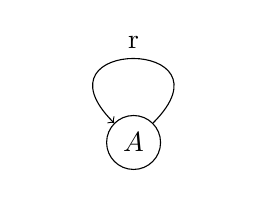
\begin{tikzpicture}
      \node[circle, draw] (A) {$A$};
      \draw[->] (A) edge[looseness=8] node[midway, above] {r} (A);
    \end{tikzpicture}
  \end{center}
  The unravelling of $G_C$ is then the graph $G_\infty$ which corresponds to the following
  picture
  \begin{center}
    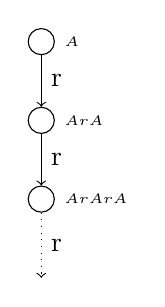
\begin{tikzpicture}
      \path{
        node[circle, draw, label=right:{\tiny$A$}] (A1) at (0,0) {}
        node[circle, draw, label=right:{\tiny$A r A$}]
        (A2) at (0,-1) {}
        node[circle, draw, label=right:{\tiny$A r A r A$}]
        (A3) at (0,-2) {}
        node[coordinate] (and so on) at (0,-3) {}
        %% 
        (A1) edge[->] node[midway, auto] {r} (A2)
        (A2) edge[->] node[midway, auto] {r} (A3)
        (A3) edge[dotted, ->] node[midway, auto] {r} (and so on)
      };
    \end{tikzpicture}
  \end{center}
  where the path to which every node corresponds is depicted right of the node.  Then, for
  $d = 3$, the unravelling of $G_C$ up to depth $3$ would just be the graph
  \begin{center}
    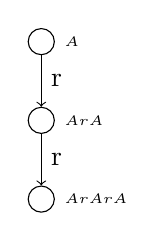
\begin{tikzpicture}
      \path{
        node[circle, draw, label=right:{\tiny$A$}] (A1) at (0,0) {}
        node[circle, draw, label=right:{\tiny$A r A$}]
        (A2) at (0,-1) {}
        node[circle, draw, label=right:{\tiny$A r A r A$}]
        (A3) at (0,-2) {}
        %% 
        (A1) edge[->] node[midway, auto] {r} (A2)
        (A2) edge[->] node[midway, auto] {r} (A3)
      };
    \end{tikzpicture}
  \end{center}
  and the corresponding \ELbot concept description is
  \begin{equation*}
    C_3 = \exists r. \exists r. \exists r. \top.
  \end{equation*}
\end{Example}

%%% Local Variables: 
%%% mode: latex
%%% TeX-master: "../main"
%%% End: 

%  LocalWords:  ELbot
